\scanpage{66}
% block: gerbe class
\[
\handwritten{\xi\in}H^{\handwritten{2}}(k_{\mathrm{pl}},G)
\]
is the class of the Tannakian gerbe which defines $\handwritten{\unsure{\deleted{\mathcal{A}}\mathcal{M}|\deleted{\mathcal{M}}\mathcal{A}|\mathcal{M}}}$. Thus knowledge of the numerical character of $\handwritten{\mathcal{M}}$ is equivalent to giving, in addition \unsure{to the|to|da}\\ \hspace*{3cm}\deleted{\inserted{(which already implies giving}}\\ group of multiplicative type $G$ over $k$, the classes $u_{\unsure{\deleted{\illegible{1}}\handwritten{*}|\handwritten{\sigma}}}(\handwritten{\xi})$ for all homomorphisms $u$ from $G$ into tori of the form $\handwritten{\prod}_{Z/k}\underline{G}_m$, where $Z$ is a finite extension of $k$. \deleted{(}We have indeed just seen that giving the numerical character makes it possible to reconstruct what precedes. To see the converse, note that \deleted{if} the rank $\unsure{\deleted{d}n|\deleted{n}d}(\handwritten{\deleted{\unsure{\xi}}\sigma})$ of $M_{\handwritten{\sigma}}$ is determined by the formula
\[
n(\handwritten{\sigma})=\operatorname{card}(\handwritten{\sigma})\operatorname{\unsure{\deleted{d}o|\deleted{o}d}rd}(\handwritten{\xi_\sigma})
\]
(where $\operatorname{card}\handwritten{\sigma}$ is the cardinality of the orbit $\handwritten{\sigma}$, $\operatorname{ord}(\handwritten{\xi_\sigma})$ is the order of $\handwritten{\xi_\sigma}$ in $\operatorname{Br}(Z_{\handwritten{\sigma}})$).

% block: determination question
The question whether the numerical character determines up to equivalence of Tannakian categories thus amounts, for fixed $G$, to the question whether an element \deleted{of} $\handwritten{\xi\in}H^{\handwritten{2}}(k_{\mathrm{pl}},G_{\deleted{\times}})$ is known when one knows the $u_{\handwritten{*}}(\handwritten{\xi})$ for $u:G\handwritten{\unsure{\mathrel{\begin{tikzpicture}[x=1cm,y=1cm,baseline=-.05cm]\draw[thin] (0,0)--(.5,0)--(.47,.12);\end{tikzpicture}}|\longrightarrow}}\underline{Z}^{\unsure{\times|x|\mathbb{x}|*}}$ as above. \deleted{We shall e\unsure{t|x|i}e\unsure{s}} This is the case for diagonalizable $G$ \deleted{pro-countable} (pro-countable ?). We shall examine two other cases.

% block: example 1
\uline{Example} \unsure{$\mathbb{I}$|I|1}. $G$ is a torus of dimension 1, hence (if it is not trivial) twisted by a quadratic extension $Z$ of $k$. We thus have an exact sequence
\diagram{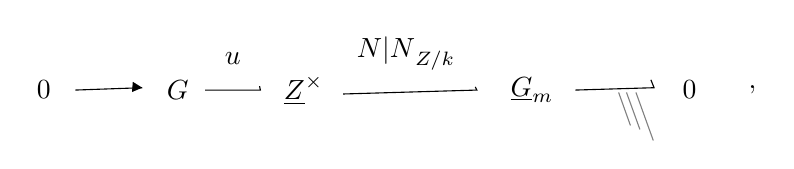
\begin{tikzpicture}[x=1cm,y=1cm]
\node at (0,0) {$0$};\node at (1.7,0) {$G$};\node at (3.3,0) {$\underline{Z}^{\times}$};\node at (6.2,0) {$\underline{G}_m$};\node at (8.2,0) {$0$};\node at (9,0) {$,$};
\draw[thin] (.4,0)--(1.25,.03);\fill (1.12,-.025)--(1.25,.03)--(1.13,.105)--cycle;
\draw[thin] (2.05,0)--(2.75,0)--(2.74,.05);\node at (2.4,.4) {$u$};
\draw[thin] (3.8,-.05)--(5.5,0)--(5.48,.04);\node at (4.6,.46) {$\unsure{\mathbb{N}|N}_{Z/k}$};
\draw[thin] (6.75,0)--(7.75,.03)--(7.71,.13);
\draw[thin,gray] (7.3,-.03)--(7.45,-.45);\draw[thin,gray] (7.4,-.03)--(7.57,-.5);\draw[thin,gray] (7.52,-.03)--(7.74,-.64);
\end{tikzpicture}}
from which we conclude, by the cohomology exact sequence and theorem 90 that $\operatorname{Ker}(u:H^{\handwritten{2}}(k,G)\handwritten{\longrightarrow}H^{\handwritten{2}}(\unsure{\deleted{i}k|\deleted{k}i},\underline{Z}^{\times}))$ is zero. Thus in the case considered, the numerical character determines $\handwritten{\mathcal{M}}$ up to equivalence.

% block: cancelled example 2
\deleted{\uline{Example} 2. Let us keep \deleted{l\unsure{'|i|t}e} $G$ as above, let $n$ be an integer $\quad2$, and let $G'=\operatorname{Ker}n.\operatorname{id}_G$. The exact sequence}
\diagram{\begin{tikzcd}[ampersand replacement=\&]
\deleted{0} \& \deleted{G'} \& \deleted{G} \arrow[r,phantom,"\deleted{n}"] \& \deleted{G} \& \deleted{0}
\end{tikzcd}}
\deleted{and the preceding result shows that the set of classes of}
\figure{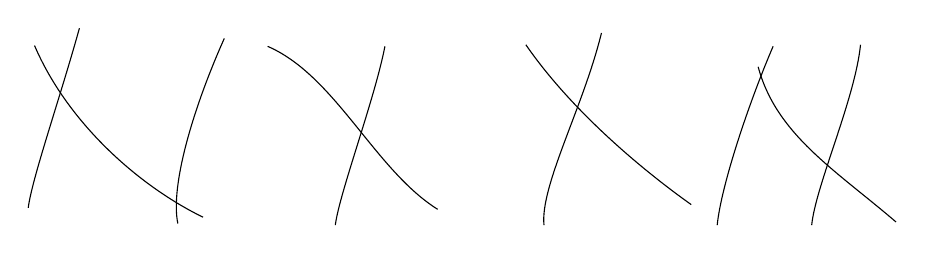
\begin{tikzpicture}[x=1cm,y=1cm]
\draw[thin] (.95,2.4).. controls (.7,1.5) and (.35,.5)..(.3,.12);
\draw[thin] (.38,2.18).. controls (.8,1.2) and (1.7,.4)..(2.52,0);
\draw[thin] (2.79,2.27).. controls (2.4,1.4) and (2.1,.4)..(2.2,-.08);
\draw[thin] (3.34,2.17).. controls (4.2,1.8) and (4.7,.6)..(5.5,.1);
\draw[thin] (4.83,2.17).. controls (4.7,1.5) and (4.25,.3)..(4.2,-.1);
\draw[thin] (6.62,2.19).. controls (7.2,1.35) and (8.1,.6)..(8.72,.16);
\draw[thin] (7.58,2.34).. controls (7.35,1.4) and (6.8,.4)..(6.85,-.1);
\draw[thin] (9.76,2.17).. controls (9.45,1.45) and (9.1,.4)..(9.05,-.1);
\draw[thin] (9.57,1.91).. controls (9.8,1.05) and (10.55,.6)..(11.32,-.06);
\draw[thin] (10.87,2.19).. controls (10.8,1.5) and (10.3,.4)..(10.25,-.1);
\end{tikzpicture}}
% archive sheet number: 65
